\section{Denial-of-Service (DoS)}

Gli attacchi di tipo Denial-of-Service (DoS) sono una tipologia di attacchi informatici estremamente diffusa, la cui
frequenza è cresciuta negli anni sia in termini quantitativi che qualitativi. Questo incremento è stato determinato
dalla relativa facilità con cui è possibile condurre un attacco di questo tipo, nonché dalle sue conseguenze, che in
base alle contromisure adottate e alla struttura del servizio attaccato possono essere più o meno gravi. Nella tesi ci
concentreremo solamente, sull’analisi della metodologia di protezione denominate rate-limiting. Queste strategie possono
risultare estremamente efficaci in alcune situazioni, come dimostrato dall’evento accaduto ad agosto 2022 a Google \cite{google_ddos},
la quale grazie all’attivazione di un rate-limiter è stata in grado di contrastare con successo il più grande attacco di tipo
DDoS a livello applicativo mai registrato. Tale attacco, proveniente da oltre 5.256 sorgenti IP dislocate in 132 paesi
differenti, ha raggiunto il picco di 46 milioni di richieste al secondo. 

In generale, un una regola per il rate-limiting consiste in un semplice conteggio delle occorrenze delle richieste in un
lasso di tempo. Tuttavia, esistono diverse tecniche per misurare e limitare la frequenza di tali richieste, ognuna con i
propri usi e implicazioni.
\begin{itemize}
    \item \textbf{Fixed window}: Tra tutte le strategie che vedremo è la più semplice da implementare, consiste nello stabilire un
    limite massimo al numero di richieste che possono essere inviate in un determinato intervallo di tempo, detto
    "finestra". Ad esempio, si potrebbe limitare il numero di richieste a 100 ogni minuto. Questo limite viene applicato in
    modo uniforme all'interno della finestra temporale. Ciò significa che, una volta raggiunto il limite massimo di
    richieste consentite, l'utente o l'applicazione deve attendere il termine della finestra temporale per poter inviare
    nuove richieste. Uno svantaggio significativo di questa strategia è la possibile concentrazione di richieste tutte in
    una porzione della finestra, rischiando un sovraccarico del servizio. Caso notevole è il caso in cui si concentrino tutte
    le richieste di una finestra al margine della fine e tutte le richieste della finestra successiva al margine dell’inizio
    questo comporta che il sistema in una durata equivalente a quella della finestra, gestisca il doppio delle richieste
    consentite.
    \begin{figure}[H]
        \centering
        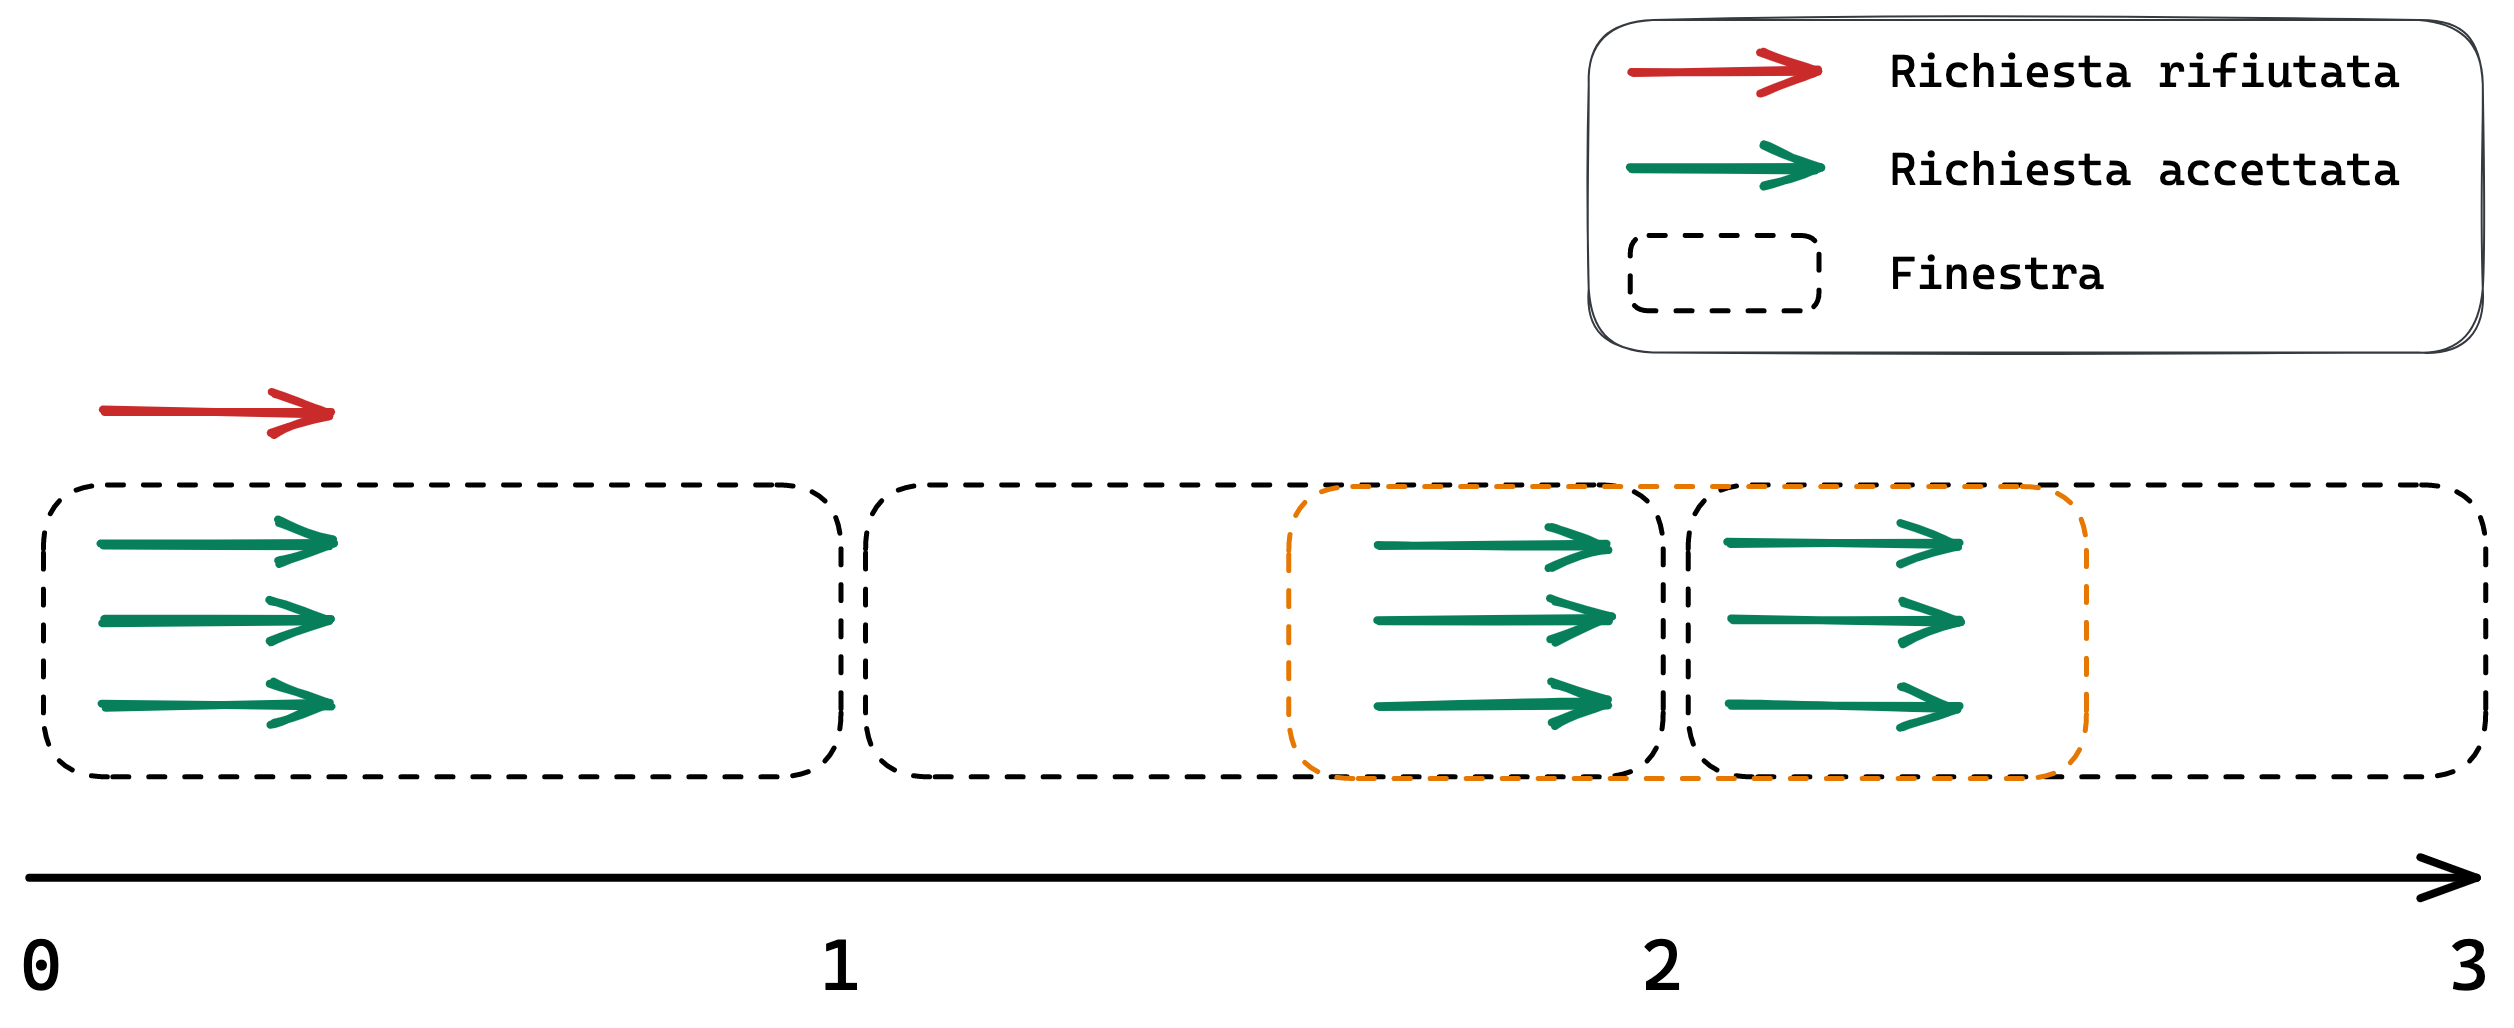
\includegraphics[width=13cm]{./chapters/1.state-of-art/images/1.fixed_window.png}
        \label{fig:fixed-window}
        \captionsetup{justification=centering}
        \caption{Strategia di rate-limiting: Fixed window}
    \end{figure}
    \item \textbf{Token bucket}: Il funzionamento del token bucket prevede che non tutte le richieste di un servizio vengano mappate
    1:1 con la richiesta di risorse, poiché alcune richieste potrebbero richiedere più risorse di altre. Per questo motivo,
    viene mantenuto un contatore di risorse, che viene scalato per ogni richiesta, del numero di token necessari per portare
    a termine il lavoro. Il contatore ha una frequenza di riempimento, ovvero a ogni unità di tempo viene reimpostato al suo
    valore massimo. Quando un utente o un'applicazione invia una richiesta al sistema, il sistema verifica se ci sono
    abbastanza token disponibili per soddisfare la richiesta. Se non ci sono abbastanza token, la richiesta viene respinta.
    In questo modo, le richieste vengono accettate solo se c'è abbastanza capacità per soddisfarle.
    \begin{figure}[h]
        \centering
        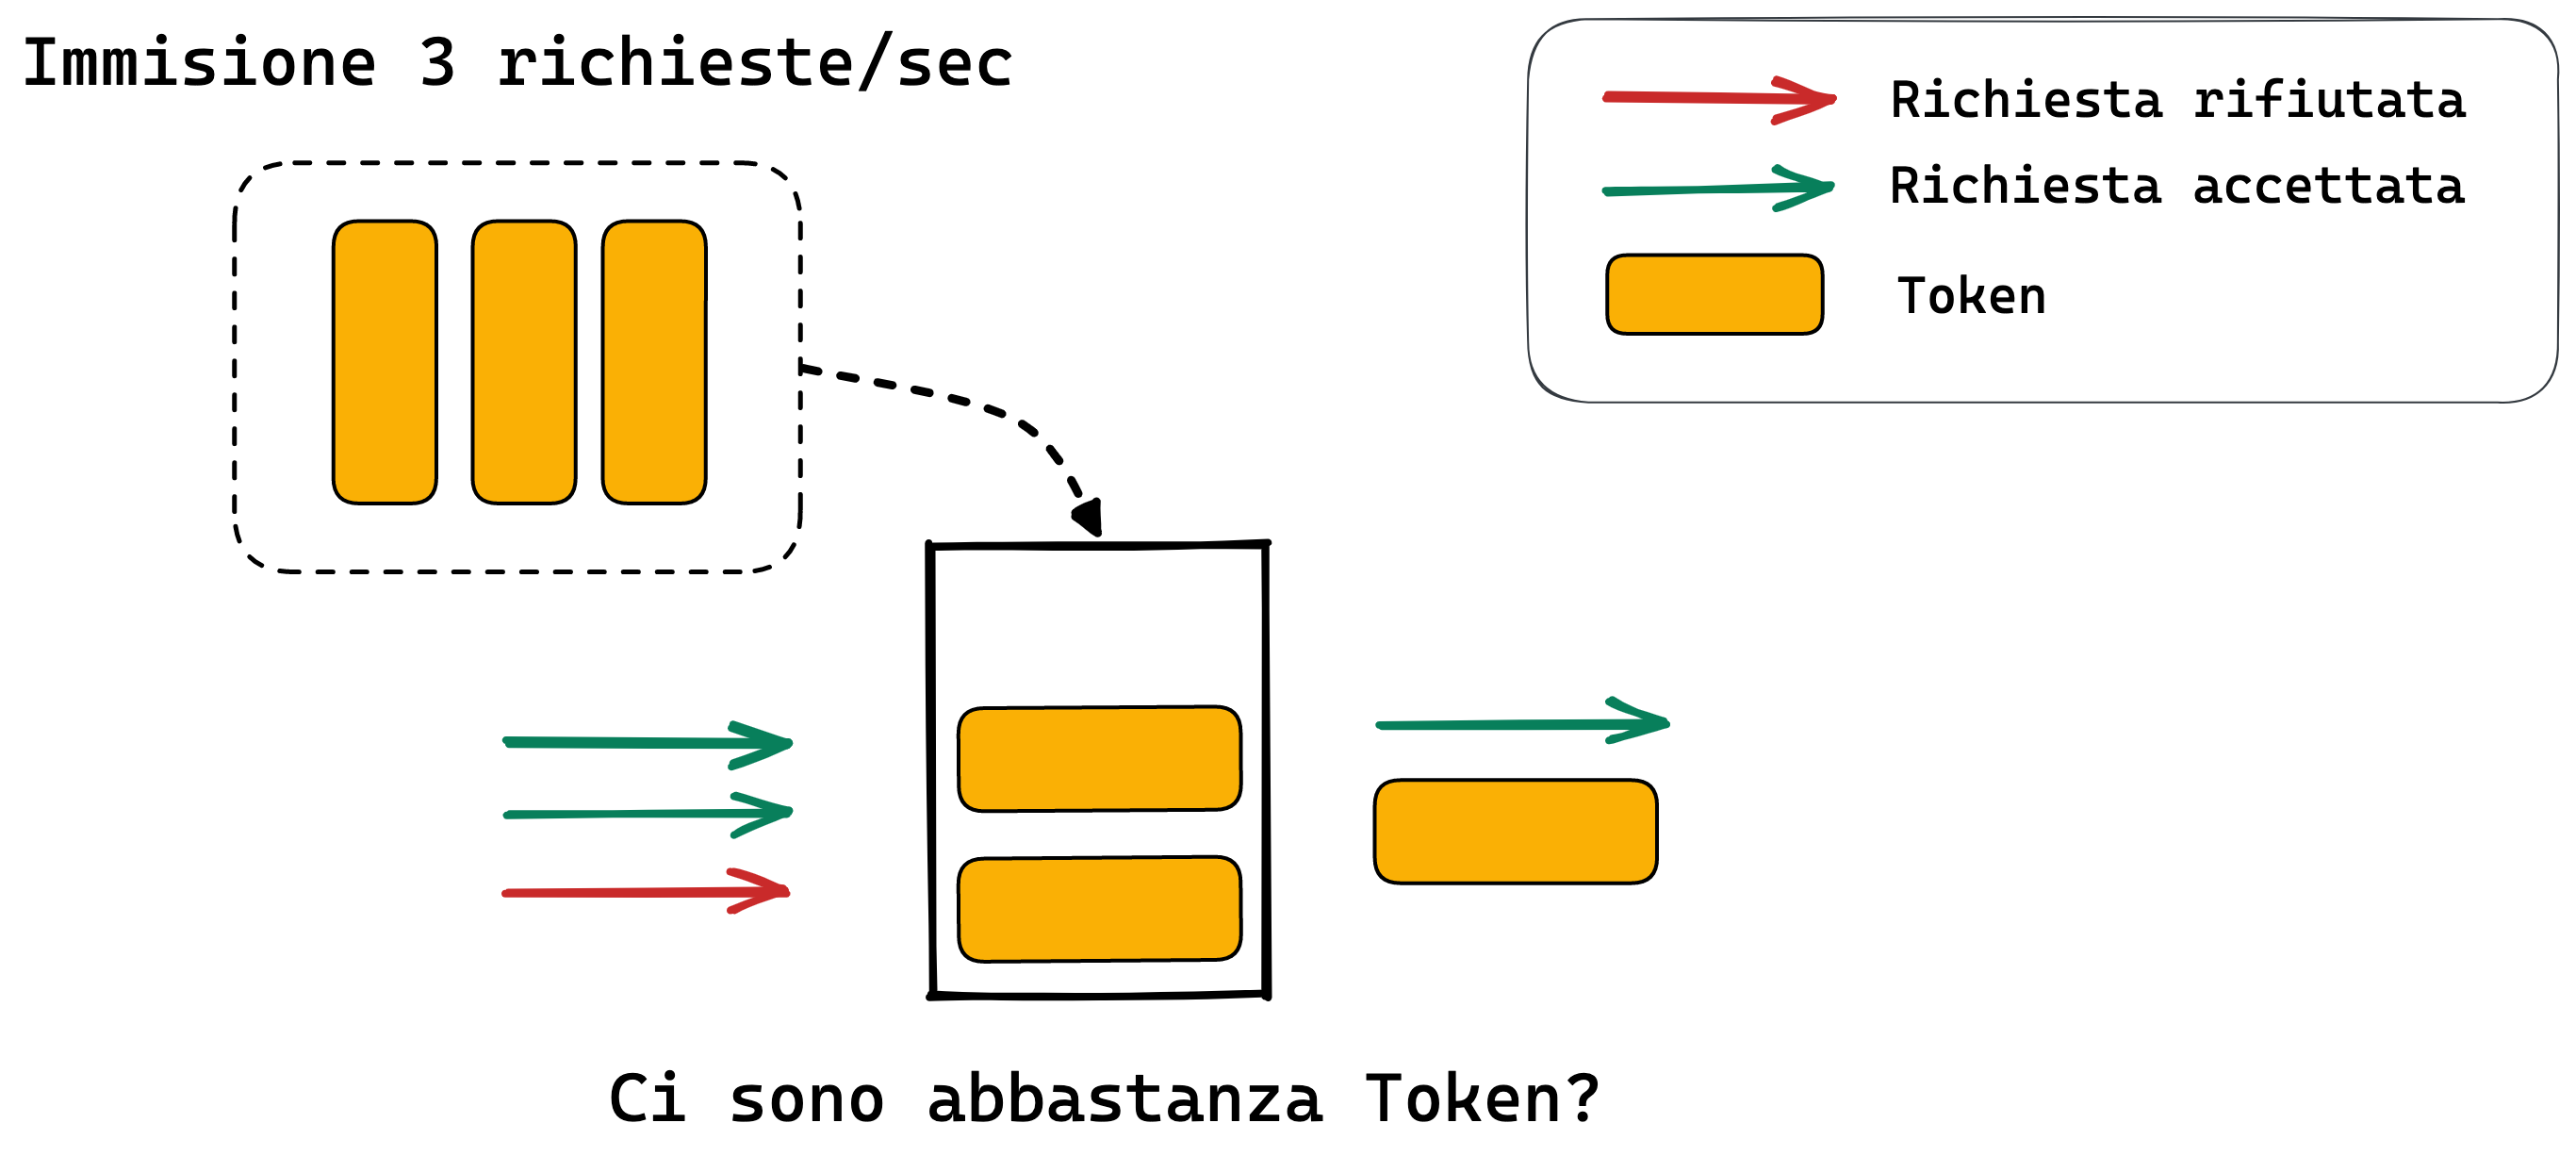
\includegraphics[width=13cm]{./chapters/1.state-of-art/images/2.token_bucket.png}
        \label{fig:token-bucket}
        \captionsetup{justification=centering}
        \caption{Strategia di rate-limiting: Token bucket}
    \end{figure}
    \item \textbf{Leaky bucket}: L'idea di base è simile a quella del Token bucket ma invece di rispondere al numero di richieste
    liberando i token necessari fino a esaurimento, il tasso di elaborazione delle richieste viene regolato in modo
    uniforme. Questo significa che quando un pacchetto di dati arriva al sistema, se il secchio (la struttura dati) è già pieno, il pacchetto
    viene scartato. Nel mentre ad ogni unità di tempo viene elaborata una quantità di richieste corrispondente alla velocità
    di uscita del sistema. In questo modo, il flusso di dati in uscita non supera mai una certa soglia.
    \begin{figure}[h]
        \centering
        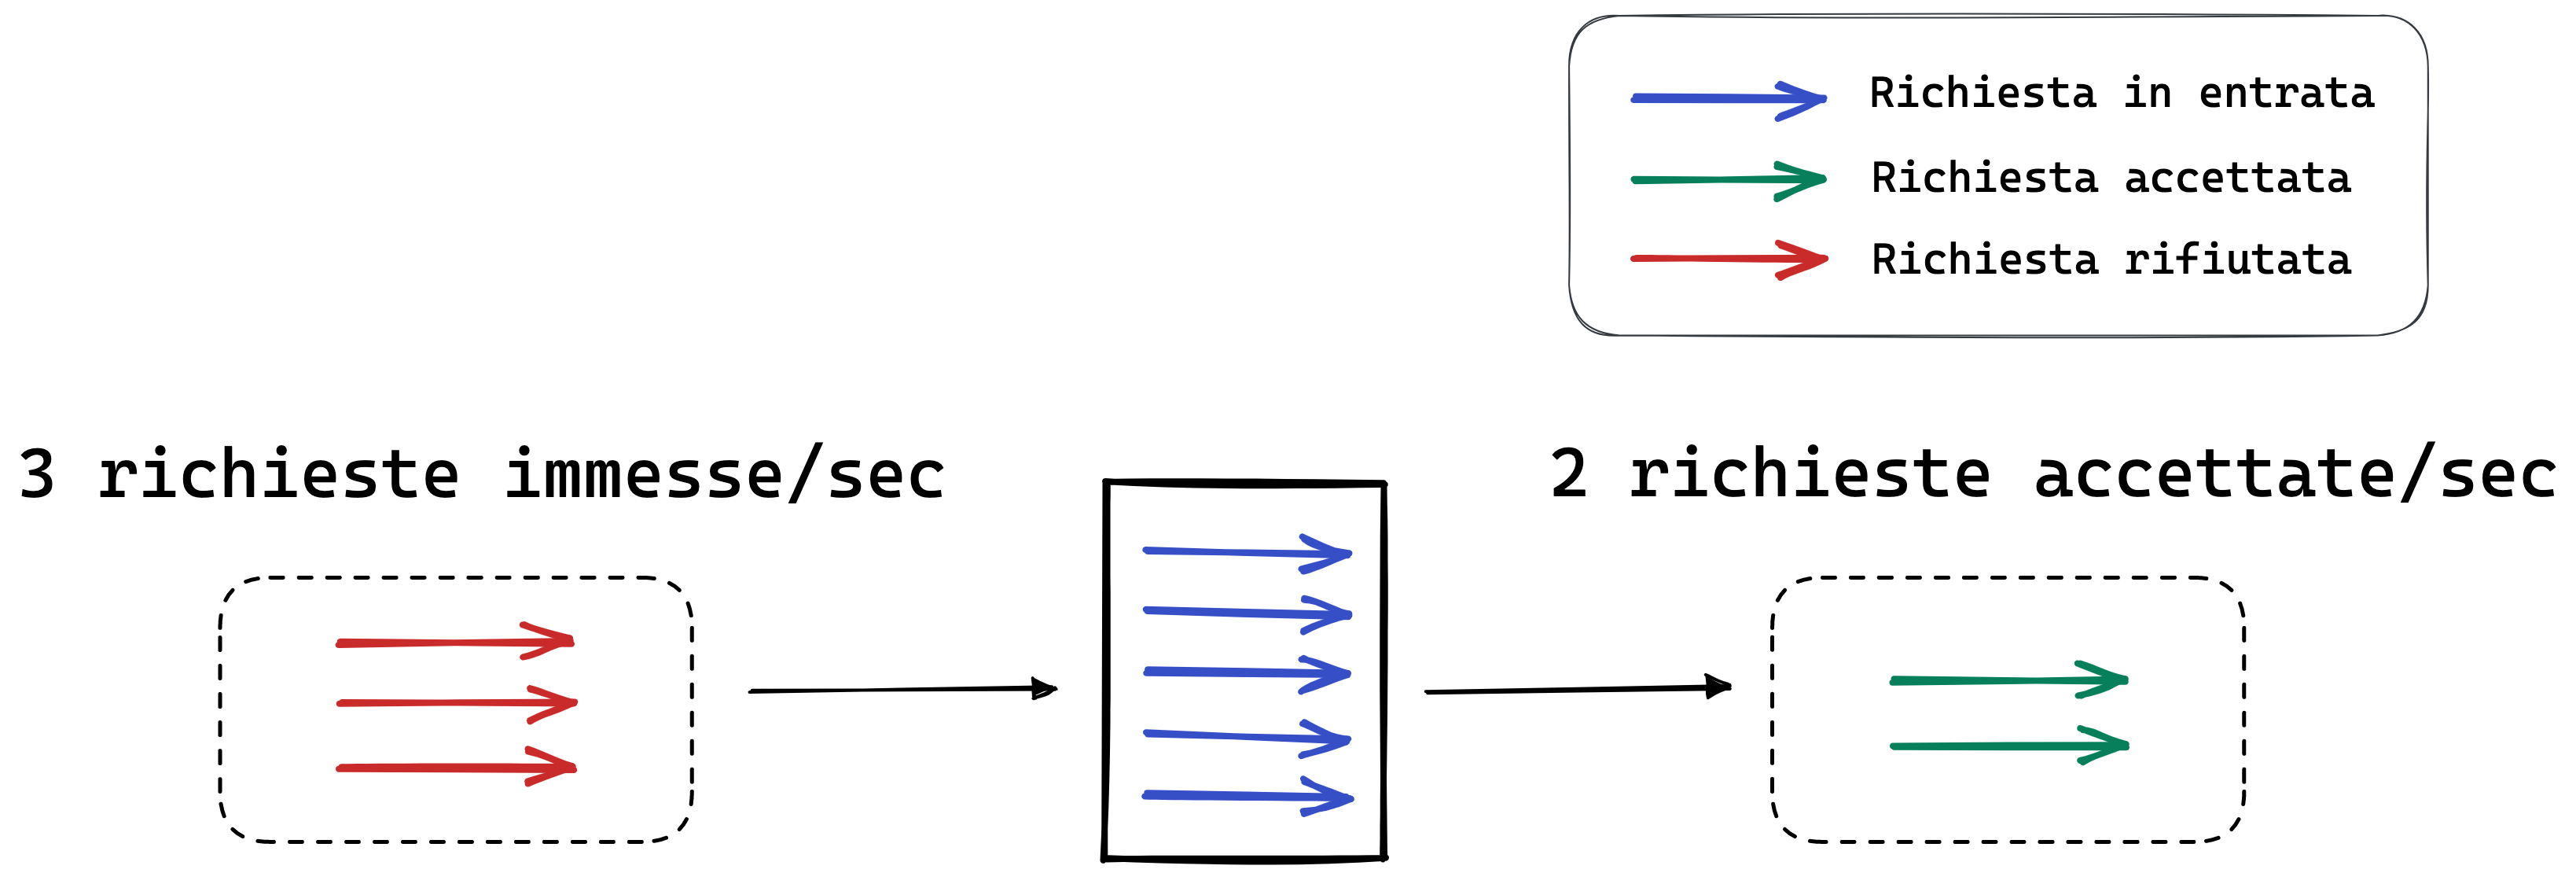
\includegraphics[width=13cm]{./chapters/1.state-of-art/images/3.leaky_bucket.png}
        \label{fig:laky-bucket}
        \captionsetup{justification=centering}
        \caption{Strategia di rate-limiting: Leaky bucket}
    \end{figure}
    \item \textbf{Sliding window}: La strategia di sliding window adotta un approccio simile alla Fixed Window, ma con una differenza
    fondamentale: esamina il tasso di richieste effettuate in un periodo di tempo continuo, piuttosto che in intervalli
    fissi. Ad esempio, se il limite di richieste è fissato a 100 al minuto, la strategia prevede di controllare il numero di
    richieste effettuate nell'ultimo minuto e, nel caso superi il limite, rifiutare la richiesta. Questo approccio evita il
    potenziale sovraccarico del sistema alla fine di una finestra con un tempo prefissato, ma richiede la gestione di una
    finestra scorrevole, aumentando la complessità di implementazione.
    \begin{figure}[h]
        \centering
        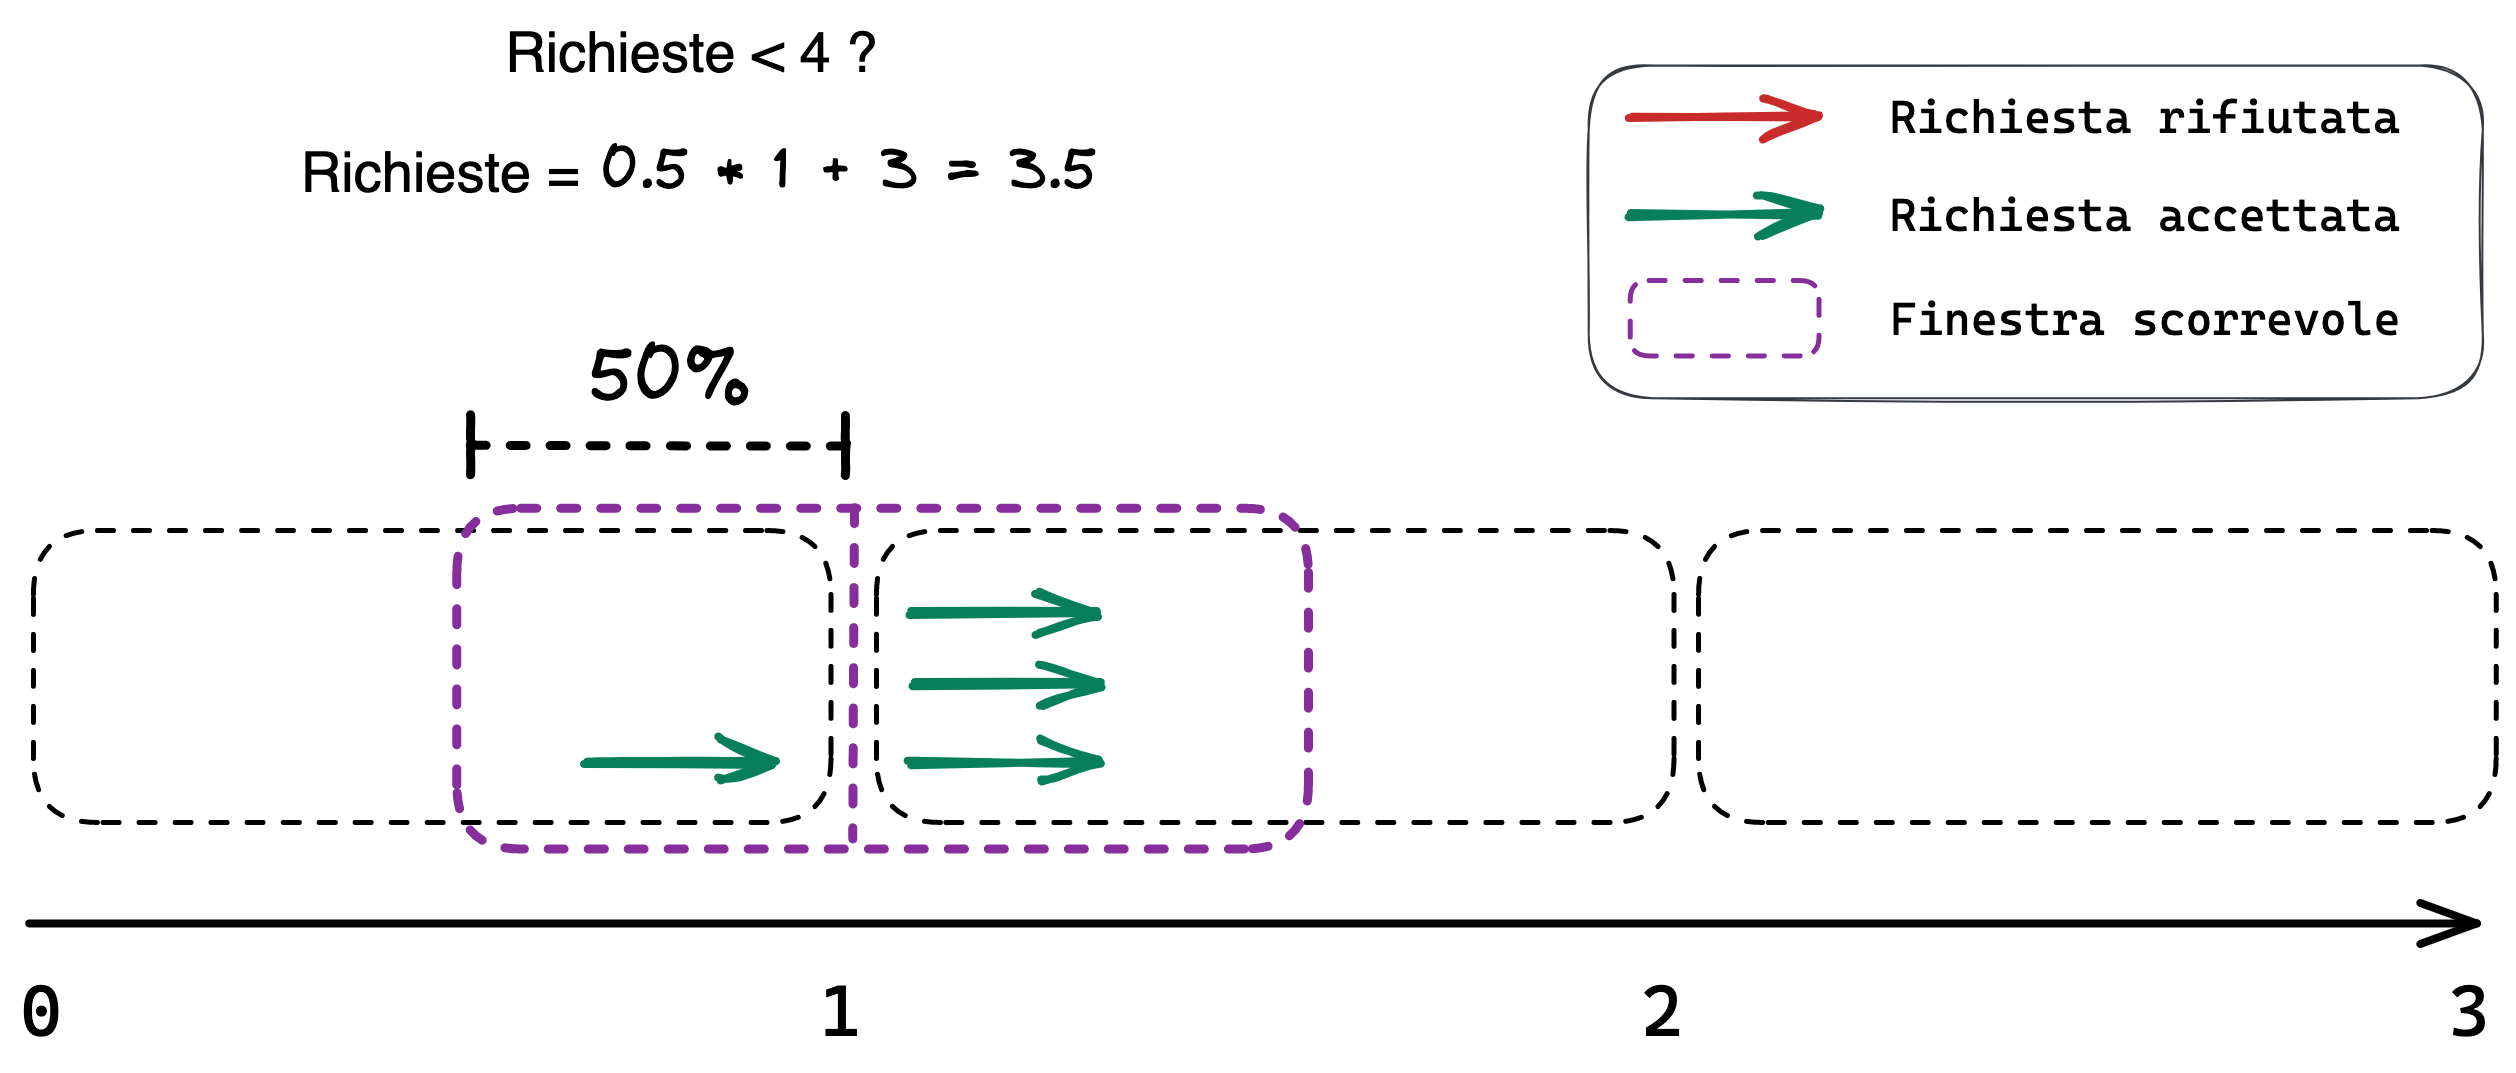
\includegraphics[width=13cm]{./chapters/1.state-of-art/images/4.sliding_window.png}
        \label{fig:sliding-window}
        \captionsetup{justification=centering}
        \caption{Strategia di rate-limiting: Sliding window}
    \end{figure}
\end{itemize}

Vale la pena notare che pur essendo un metodo ampiamente utilizzato il rate-limiting da solo potrebbe risultare
insufficiente per garantire un livello di sicurezza adeguato, contro gli attacchi DoS, pertanto è necessario adottare
contromisure di diversa natura, al fine di garantire una protezione completa.